\documentclass[1p]{elsarticle_modified}
%\bibliographystyle{elsarticle-num}

%\usepackage[colorlinks]{hyperref}
%\usepackage{abbrmath_seonhwa} %\Abb, \Ascr, \Acal ,\Abf, \Afrak
\usepackage{amsfonts}
\usepackage{amssymb}
\usepackage{amsmath}
\usepackage{amsthm}
\usepackage{scalefnt}
\usepackage{amsbsy}
\usepackage{kotex}
\usepackage{caption}
\usepackage{subfig}
\usepackage{color}
\usepackage{graphicx}
\usepackage{xcolor} %% white, black, red, green, blue, cyan, magenta, yellow
\usepackage{float}
\usepackage{setspace}
\usepackage{hyperref}

\usepackage{tikz}
\usetikzlibrary{arrows}

\usepackage{multirow}
\usepackage{array} % fixed length table
\usepackage{hhline}

%%%%%%%%%%%%%%%%%%%%%
\makeatletter
\renewcommand*\env@matrix[1][\arraystretch]{%
	\edef\arraystretch{#1}%
	\hskip -\arraycolsep
	\let\@ifnextchar\new@ifnextchar
	\array{*\c@MaxMatrixCols c}}
\makeatother %https://tex.stackexchange.com/questions/14071/how-can-i-increase-the-line-spacing-in-a-matrix
%%%%%%%%%%%%%%%

\usepackage[normalem]{ulem}

\newcommand{\msout}[1]{\ifmmode\text{\sout{\ensuremath{#1}}}\else\sout{#1}\fi}
%SOURCE: \msout is \stkout macro in https://tex.stackexchange.com/questions/20609/strikeout-in-math-mode

\newcommand{\cancel}[1]{
	\ifmmode
	{\color{red}\msout{#1}}
	\else
	{\color{red}\sout{#1}}
	\fi
}

\newcommand{\add}[1]{
	{\color{blue}\uwave{#1}}
}

\newcommand{\replace}[2]{
	\ifmmode
	{\color{red}\msout{#1}}{\color{blue}\uwave{#2}}
	\else
	{\color{red}\sout{#1}}{\color{blue}\uwave{#2}}
	\fi
}

\newcommand{\Sol}{\mathcal{S}} %segment
\newcommand{\D}{D} %diagram
\newcommand{\A}{\mathcal{A}} %arc


%%%%%%%%%%%%%%%%%%%%%%%%%%%%%5 test

\def\sl{\operatorname{\textup{SL}}(2,\Cbb)}
\def\psl{\operatorname{\textup{PSL}}(2,\Cbb)}
\def\quan{\mkern 1mu \triangleright \mkern 1mu}

\theoremstyle{definition}
\newtheorem{thm}{Theorem}[section]
\newtheorem{prop}[thm]{Proposition}
\newtheorem{lem}[thm]{Lemma}
\newtheorem{ques}[thm]{Question}
\newtheorem{cor}[thm]{Corollary}
\newtheorem{defn}[thm]{Definition}
\newtheorem{exam}[thm]{Example}
\newtheorem{rmk}[thm]{Remark}
\newtheorem{alg}[thm]{Algorithm}

\newcommand{\I}{\sqrt{-1}}
\begin{document}

%\begin{frontmatter}
%
%\title{Boundary parabolic representations of knots up to 8 crossings}
%
%%% Group authors per affiliation:
%\author{Yunhi Cho} 
%\address{Department of Mathematics, University of Seoul, Seoul, Korea}
%\ead{yhcho@uos.ac.kr}
%
%
%\author{Seonhwa Kim} %\fnref{s_kim}}
%\address{Center for Geometry and Physics, Institute for Basic Science, Pohang, 37673, Korea}
%\ead{ryeona17@ibs.re.kr}
%
%\author{Hyuk Kim}
%\address{Department of Mathematical Sciences, Seoul National University, Seoul 08826, Korea}
%\ead{hyukkim@snu.ac.kr}
%
%\author{Seokbeom Yoon}
%\address{Department of Mathematical Sciences, Seoul National University, Seoul, 08826,  Korea}
%\ead{sbyoon15@snu.ac.kr}
%
%\begin{abstract}
%We find all boundary parabolic representation of knots up to 8 crossings.
%
%\end{abstract}
%\begin{keyword}
%    \MSC[2010] 57M25 
%\end{keyword}
%
%\end{frontmatter}

%\linenumbers
%\tableofcontents
%
\newcommand\colored[1]{\textcolor{white}{\rule[-0.35ex]{0.8em}{1.4ex}}\kern-0.8em\color{red} #1}%
%\newcommand\colored[1]{\textcolor{white}{ #1}\kern-2.17ex	\textcolor{white}{ #1}\kern-1.81ex	\textcolor{white}{ #1}\kern-2.15ex\color{red}#1	}

{\Large $\underline{12n_{0766}~(K12n_{0766})}$}

\setlength{\tabcolsep}{10pt}
\renewcommand{\arraystretch}{1.6}
\vspace{1cm}\begin{tabular}{m{100pt}>{\centering\arraybackslash}m{274pt}}
\multirow{5}{120pt}{
	\centering
	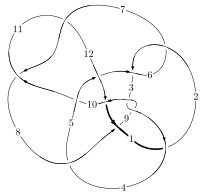
\includegraphics[width=112pt]{../../../GIT/diagram.site/Diagrams/png/2855_12n_0766.png}\\
\ \ \ A knot diagram\footnotemark}&
\allowdisplaybreaks
\textbf{Linearized knot diagam} \\
\cline{2-2}
 &
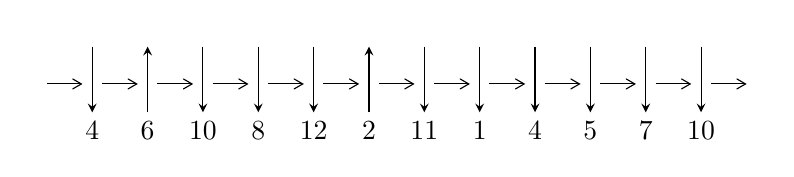
\begin{tikzpicture}[x=20pt, y=17pt]
	% nodes
	\node (C0) at (0, 0) {};
	\node (C1) at (1, 0) {};
	\node (C1U) at (1, +1) {};
	\node (C1D) at (1, -1) {4};

	\node (C2) at (2, 0) {};
	\node (C2U) at (2, +1) {};
	\node (C2D) at (2, -1) {6};

	\node (C3) at (3, 0) {};
	\node (C3U) at (3, +1) {};
	\node (C3D) at (3, -1) {10};

	\node (C4) at (4, 0) {};
	\node (C4U) at (4, +1) {};
	\node (C4D) at (4, -1) {8};

	\node (C5) at (5, 0) {};
	\node (C5U) at (5, +1) {};
	\node (C5D) at (5, -1) {12};

	\node (C6) at (6, 0) {};
	\node (C6U) at (6, +1) {};
	\node (C6D) at (6, -1) {2};

	\node (C7) at (7, 0) {};
	\node (C7U) at (7, +1) {};
	\node (C7D) at (7, -1) {11};

	\node (C8) at (8, 0) {};
	\node (C8U) at (8, +1) {};
	\node (C8D) at (8, -1) {1};

	\node (C9) at (9, 0) {};
	\node (C9U) at (9, +1) {};
	\node (C9D) at (9, -1) {4};

	\node (C10) at (10, 0) {};
	\node (C10U) at (10, +1) {};
	\node (C10D) at (10, -1) {5};

	\node (C11) at (11, 0) {};
	\node (C11U) at (11, +1) {};
	\node (C11D) at (11, -1) {7};

	\node (C12) at (12, 0) {};
	\node (C12U) at (12, +1) {};
	\node (C12D) at (12, -1) {10};
	\node (C13) at (13, 0) {};

	% arrows
	\draw[->,>={angle 60}]
	(C0) edge (C1) (C1) edge (C2) (C2) edge (C3) (C3) edge (C4) (C4) edge (C5) (C5) edge (C6) (C6) edge (C7) (C7) edge (C8) (C8) edge (C9) (C9) edge (C10) (C10) edge (C11) (C11) edge (C12) (C12) edge (C13) ;	\draw[->,>=stealth]
	(C1U) edge (C1D) (C2D) edge (C2U) (C3U) edge (C3D) (C4U) edge (C4D) (C5U) edge (C5D) (C6D) edge (C6U) (C7U) edge (C7D) (C8U) edge (C8D) (C9U) edge (C9D) (C10U) edge (C10D) (C11U) edge (C11D) (C12U) edge (C12D) ;
	\end{tikzpicture} \\
\hhline{~~} \\& 
\textbf{Solving Sequence} \\ \cline{2-2} 
 &
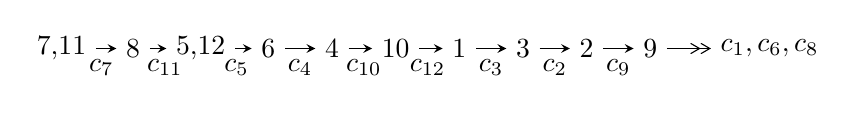
\begin{tikzpicture}[x=23pt, y=7pt]
	% node
	\node (A0) at (-1/8, 0) {7,11};
	\node (A1) at (1, 0) {8};
	\node (A2) at (33/16, 0) {5,12};
	\node (A3) at (25/8, 0) {6};
	\node (A4) at (33/8, 0) {4};
	\node (A5) at (41/8, 0) {10};
	\node (A6) at (49/8, 0) {1};
	\node (A7) at (57/8, 0) {3};
	\node (A8) at (65/8, 0) {2};
	\node (A9) at (73/8, 0) {9};
	\node (C1) at (1/2, -1) {$c_{7}$};
	\node (C2) at (3/2, -1) {$c_{11}$};
	\node (C3) at (21/8, -1) {$c_{5}$};
	\node (C4) at (29/8, -1) {$c_{4}$};
	\node (C5) at (37/8, -1) {$c_{10}$};
	\node (C6) at (45/8, -1) {$c_{12}$};
	\node (C7) at (53/8, -1) {$c_{3}$};
	\node (C8) at (61/8, -1) {$c_{2}$};
	\node (C9) at (69/8, -1) {$c_{9}$};
	\node (A10) at (11, 0) {$c_{1},c_{6},c_{8}$};

	% edge
	\draw[->,>=stealth]	
	(A0) edge (A1) (A1) edge (A2) (A2) edge (A3) (A3) edge (A4) (A4) edge (A5) (A5) edge (A6) (A6) edge (A7) (A7) edge (A8) (A8) edge (A9) ;
	\draw[->>,>={angle 60}]	
	(A9) edge (A10);
\end{tikzpicture} \\ 

\end{tabular} \\

\footnotetext{
The image of knot diagram is generated by the software ``\textbf{Draw programme}" developed by Andrew Bartholomew(\url{http://www.layer8.co.uk/maths/draw/index.htm\#Running-draw}), where we modified some parts for our purpose(\url{https://github.com/CATsTAILs/LinksPainter}).
}\phantom \\ \newline 
\centering \textbf{Ideals for irreducible components\footnotemark of $X_{\text{par}}$} 
 
\begin{align*}
I^u_{1}&=\langle 
4.30257\times10^{223} u^{73}-1.59534\times10^{224} u^{72}+\cdots+3.52832\times10^{224} b-2.38648\times10^{226},\\
\phantom{I^u_{1}}&\phantom{= \langle  }-1.18385\times10^{227} u^{73}+4.85389\times10^{227} u^{72}+\cdots+1.03768\times10^{228} a+1.60594\times10^{229},\\
\phantom{I^u_{1}}&\phantom{= \langle  }2 u^{74}-7 u^{73}+\cdots-16845 u-2941\rangle \\
I^u_{2}&=\langle 
-3.25053\times10^{21} u^{25}-6.44125\times10^{21} u^{24}+\cdots+2.54323\times10^{21} b-7.68603\times10^{21},\\
\phantom{I^u_{2}}&\phantom{= \langle  }4.00630\times10^{22} u^{25}+4.85877\times10^{22} u^{24}+\cdots+1.27162\times10^{22} a-9.79215\times10^{22},\;2 u^{26}+3 u^{25}+\cdots+3 u+5\rangle \\
\\
\end{align*}
\raggedright * 2 irreducible components of $\dim_{\mathbb{C}}=0$, with total 100 representations.\\
\footnotetext{All coefficients of polynomials are rational numbers. But the coefficients are sometimes approximated in decimal forms when there is not enough margin.}
\newpage
\renewcommand{\arraystretch}{1}
\centering \section*{I. $I^u_{1}= \langle 4.30\times10^{223} u^{73}-1.60\times10^{224} u^{72}+\cdots+3.53\times10^{224} b-2.39\times10^{226},\;-1.18\times10^{227} u^{73}+4.85\times10^{227} u^{72}+\cdots+1.04\times10^{228} a+1.61\times10^{229},\;2 u^{74}-7 u^{73}+\cdots-16845 u-2941 \rangle$}
\flushleft \textbf{(i) Arc colorings}\\
\begin{tabular}{m{7pt} m{180pt} m{7pt} m{180pt} }
\flushright $a_{7}=$&$\begin{pmatrix}1\\0\end{pmatrix}$ \\
\flushright $a_{11}=$&$\begin{pmatrix}0\\u\end{pmatrix}$ \\
\flushright $a_{8}=$&$\begin{pmatrix}1\\u^2\end{pmatrix}$ \\
\flushright $a_{5}=$&$\begin{pmatrix}0.114087 u^{73}-0.467764 u^{72}+\cdots-245.040 u-15.4763\\-0.121944 u^{73}+0.452153 u^{72}+\cdots+532.776 u+67.6377\end{pmatrix}$ \\
\flushright $a_{12}=$&$\begin{pmatrix}- u\\u\end{pmatrix}$ \\
\flushright $a_{6}=$&$\begin{pmatrix}0.0868585 u^{73}-0.413586 u^{72}+\cdots+129.619 u+47.9189\\-0.0947156 u^{73}+0.397975 u^{72}+\cdots+158.117 u+4.24257\end{pmatrix}$ \\
\flushright $a_{4}=$&$\begin{pmatrix}0.0617274 u^{73}-0.381249 u^{72}+\cdots+696.582 u+152.833\\-0.0171680 u^{73}+0.135545 u^{72}+\cdots-359.031 u-74.6220\end{pmatrix}$ \\
\flushright $a_{10}=$&$\begin{pmatrix}-0.312963 u^{73}+0.836273 u^{72}+\cdots+3468.82 u+582.248\\0.351363 u^{73}-0.929137 u^{72}+\cdots-4120.61 u-695.633\end{pmatrix}$ \\
\flushright $a_{1}=$&$\begin{pmatrix}0.286378 u^{73}-1.50591 u^{72}+\cdots+2610.83 u+594.370\\-0.182080 u^{73}+1.24961 u^{72}+\cdots-3728.07 u-779.031\end{pmatrix}$ \\
\flushright $a_{3}=$&$\begin{pmatrix}0.665053 u^{73}-3.07468 u^{72}+\cdots+1842.56 u+551.877\\-0.448541 u^{73}+2.43442 u^{72}+\cdots-3955.59 u-895.987\end{pmatrix}$ \\
\flushright $a_{2}=$&$\begin{pmatrix}0.275851 u^{73}-1.31333 u^{72}+\cdots+1415.83 u+352.827\\-0.132560 u^{73}+0.746912 u^{72}+\cdots-1432.05 u-319.676\end{pmatrix}$ \\
\flushright $a_{9}=$&$\begin{pmatrix}-0.530006 u^{73}+1.62015 u^{72}+\cdots+4466.85 u+715.631\\0.503235 u^{73}-1.26199 u^{72}+\cdots-6391.55 u-1090.11\end{pmatrix}$\\&\end{tabular}
\flushleft \textbf{(ii) Obstruction class $= -1$}\\~\\
\flushleft \textbf{(iii) Cusp Shapes $= 0.310330 u^{73}-0.873656 u^{72}+\cdots-3442.04 u-587.923$}\\~\\
\newpage\renewcommand{\arraystretch}{1}
\flushleft \textbf{(iv) u-Polynomials at the component}\newline \\
\begin{tabular}{m{50pt}|m{274pt}}
Crossings & \hspace{64pt}u-Polynomials at each crossing \\
\hline $$\begin{aligned}c_{1}\end{aligned}$$&$\begin{aligned}
&2(2 u^{74}-3 u^{73}+\cdots+5635 u+1357)
\end{aligned}$\\
\hline $$\begin{aligned}c_{2},c_{6}\end{aligned}$$&$\begin{aligned}
&u^{74}-2 u^{73}+\cdots-215 u+91
\end{aligned}$\\
\hline $$\begin{aligned}c_{3},c_{9}\end{aligned}$$&$\begin{aligned}
&2(2 u^{74}+5 u^{73}+\cdots+1357162 u-1267391)
\end{aligned}$\\
\hline $$\begin{aligned}c_{4}\end{aligned}$$&$\begin{aligned}
&u^{74}+2 u^{73}+\cdots-15076 u+11221
\end{aligned}$\\
\hline $$\begin{aligned}c_{5}\end{aligned}$$&$\begin{aligned}
&u^{74}+u^{73}+\cdots+15239 u-3254
\end{aligned}$\\
\hline $$\begin{aligned}c_{7},c_{11}\end{aligned}$$&$\begin{aligned}
&2(2 u^{74}+7 u^{73}+\cdots+16845 u-2941)
\end{aligned}$\\
\hline $$\begin{aligned}c_{8}\end{aligned}$$&$\begin{aligned}
&u^{74}+u^{73}+\cdots-327620 u-108299
\end{aligned}$\\
\hline $$\begin{aligned}c_{10}\end{aligned}$$&$\begin{aligned}
&u^{74}+u^{73}+\cdots-2955 u-682
\end{aligned}$\\
\hline $$\begin{aligned}c_{12}\end{aligned}$$&$\begin{aligned}
&4(4 u^{74}-55 u^{73}+\cdots-5042508 u+189693)
\end{aligned}$\\
\hline
\end{tabular}\\~\\
\newpage\renewcommand{\arraystretch}{1}
\flushleft \textbf{(v) Riley Polynomials at the component}\newline \\
\begin{tabular}{m{50pt}|m{274pt}}
Crossings & \hspace{64pt}Riley Polynomials at each crossing \\
\hline $$\begin{aligned}c_{1}\end{aligned}$$&$\begin{aligned}
&4(4 y^{74}-365 y^{73}+\cdots-4.76298\times10^{8} y+1841449)
\end{aligned}$\\
\hline $$\begin{aligned}c_{2},c_{6}\end{aligned}$$&$\begin{aligned}
&y^{74}+44 y^{73}+\cdots+374559 y+8281
\end{aligned}$\\
\hline $$\begin{aligned}c_{3},c_{9}\end{aligned}$$&$\begin{aligned}
&4(4 y^{74}-385 y^{73}+\cdots-1.71162\times10^{13} y+1.60628\times10^{12})
\end{aligned}$\\
\hline $$\begin{aligned}c_{4}\end{aligned}$$&$\begin{aligned}
&y^{74}+42 y^{73}+\cdots+674142038 y+125910841
\end{aligned}$\\
\hline $$\begin{aligned}c_{5}\end{aligned}$$&$\begin{aligned}
&y^{74}-23 y^{73}+\cdots-131821697 y+10588516
\end{aligned}$\\
\hline $$\begin{aligned}c_{7},c_{11}\end{aligned}$$&$\begin{aligned}
&4(4 y^{74}+223 y^{73}+\cdots+5.75137\times10^{7} y+8649481)
\end{aligned}$\\
\hline $$\begin{aligned}c_{8}\end{aligned}$$&$\begin{aligned}
&y^{74}-73 y^{73}+\cdots-102167052718 y+11728673401
\end{aligned}$\\
\hline $$\begin{aligned}c_{10}\end{aligned}$$&$\begin{aligned}
&y^{74}+27 y^{73}+\cdots+11416983 y+465124
\end{aligned}$\\
\hline $$\begin{aligned}c_{12}\end{aligned}$$&$\begin{aligned}
&16(16 y^{74}-1361 y^{73}+\cdots-3.95388\times10^{12} y+3.59834\times10^{10})
\end{aligned}$\\
\hline
\end{tabular}\\~\\
\newpage\flushleft \textbf{(vi) Complex Volumes and Cusp Shapes}
$$\begin{array}{c|c|c}  
\text{Solutions to }I^u_{1}& \I (\text{vol} + \sqrt{-1}CS) & \text{Cusp shape}\\
 \hline 
\begin{aligned}
u &= -0.282540 + 0.965432 I \\
a &= \phantom{-}1.97958 - 0.61451 I \\
b &= -2.36679 + 0.10892 I\end{aligned}
 & \phantom{-}5.94493 + 1.20153 I & \phantom{-0.000000 } 0 \\ \hline\begin{aligned}
u &= -0.282540 - 0.965432 I \\
a &= \phantom{-}1.97958 + 0.61451 I \\
b &= -2.36679 - 0.10892 I\end{aligned}
 & \phantom{-}5.94493 - 1.20153 I & \phantom{-0.000000 } 0 \\ \hline\begin{aligned}
u &= -0.273716 + 0.955237 I \\
a &= \phantom{-}0.964437 + 0.589339 I \\
b &= -1.65206 - 1.31053 I\end{aligned}
 & -4.12089 + 2.31752 I & \phantom{-0.000000 } 0 \\ \hline\begin{aligned}
u &= -0.273716 - 0.955237 I \\
a &= \phantom{-}0.964437 - 0.589339 I \\
b &= -1.65206 + 1.31053 I\end{aligned}
 & -4.12089 - 2.31752 I & \phantom{-0.000000 } 0 \\ \hline\begin{aligned}
u &= \phantom{-}0.850496 + 0.543632 I \\
a &= \phantom{-}0.560041 - 0.577085 I \\
b &= \phantom{-}0.286399 + 0.141759 I\end{aligned}
 & -3.21620 - 2.62127 I & \phantom{-0.000000 } 0 \\ \hline\begin{aligned}
u &= \phantom{-}0.850496 - 0.543632 I \\
a &= \phantom{-}0.560041 + 0.577085 I \\
b &= \phantom{-}0.286399 - 0.141759 I\end{aligned}
 & -3.21620 + 2.62127 I & \phantom{-0.000000 } 0 \\ \hline\begin{aligned}
u &= \phantom{-}0.129802 + 0.975847 I \\
a &= -0.906793 - 0.098111 I \\
b &= \phantom{-}1.82693 - 1.49863 I\end{aligned}
 & \phantom{-}1.63235 - 1.32777 I & \phantom{-0.000000 } 0 \\ \hline\begin{aligned}
u &= \phantom{-}0.129802 - 0.975847 I \\
a &= -0.906793 + 0.098111 I \\
b &= \phantom{-}1.82693 + 1.49863 I\end{aligned}
 & \phantom{-}1.63235 + 1.32777 I & \phantom{-0.000000 } 0 \\ \hline\begin{aligned}
u &= \phantom{-}0.227538 + 0.989919 I \\
a &= -0.949692 + 0.421748 I \\
b &= \phantom{-}1.44010 + 0.70533 I\end{aligned}
 & -0.40348 - 4.84228 I & \phantom{-0.000000 } 0 \\ \hline\begin{aligned}
u &= \phantom{-}0.227538 - 0.989919 I \\
a &= -0.949692 - 0.421748 I \\
b &= \phantom{-}1.44010 - 0.70533 I\end{aligned}
 & -0.40348 + 4.84228 I & \phantom{-0.000000 } 0\\
 \hline 
 \end{array}$$\newpage$$\begin{array}{c|c|c}  
\text{Solutions to }I^u_{1}& \I (\text{vol} + \sqrt{-1}CS) & \text{Cusp shape}\\
 \hline 
\begin{aligned}
u &= \phantom{-}0.451986 + 0.911224 I \\
a &= -0.986328 + 0.186176 I \\
b &= \phantom{-}1.36894 - 0.72134 I\end{aligned}
 & -1.94739 - 2.05739 I & \phantom{-0.000000 } 0 \\ \hline\begin{aligned}
u &= \phantom{-}0.451986 - 0.911224 I \\
a &= -0.986328 - 0.186176 I \\
b &= \phantom{-}1.36894 + 0.72134 I\end{aligned}
 & -1.94739 + 2.05739 I & \phantom{-0.000000 } 0 \\ \hline\begin{aligned}
u &= -0.882267 + 0.418072 I \\
a &= \phantom{-}0.794732 + 0.966645 I \\
b &= \phantom{-}0.102572 + 0.568615 I\end{aligned}
 & -11.22430 - 3.31101 I & \phantom{-0.000000 } 0 \\ \hline\begin{aligned}
u &= -0.882267 - 0.418072 I \\
a &= \phantom{-}0.794732 - 0.966645 I \\
b &= \phantom{-}0.102572 - 0.568615 I\end{aligned}
 & -11.22430 + 3.31101 I & \phantom{-0.000000 } 0 \\ \hline\begin{aligned}
u &= -0.326030 + 1.001260 I \\
a &= \phantom{-}1.78729 - 0.35964 I \\
b &= -2.07467 + 0.41391 I\end{aligned}
 & \phantom{-}8.32262 + 1.34742 I & \phantom{-0.000000 } 0 \\ \hline\begin{aligned}
u &= -0.326030 - 1.001260 I \\
a &= \phantom{-}1.78729 + 0.35964 I \\
b &= -2.07467 - 0.41391 I\end{aligned}
 & \phantom{-}8.32262 - 1.34742 I & \phantom{-0.000000 } 0 \\ \hline\begin{aligned}
u &= \phantom{-}0.112227 + 0.923316 I \\
a &= -0.552088 - 1.134390 I \\
b &= \phantom{-}0.487672 - 0.685782 I\end{aligned}
 & \phantom{-}1.41563 + 0.22117 I & -8.00000 + 0. I\phantom{ +0.000000I} \\ \hline\begin{aligned}
u &= \phantom{-}0.112227 - 0.923316 I \\
a &= -0.552088 + 1.134390 I \\
b &= \phantom{-}0.487672 + 0.685782 I\end{aligned}
 & \phantom{-}1.41563 - 0.22117 I & -8.00000 + 0. I\phantom{ +0.000000I} \\ \hline\begin{aligned}
u &= \phantom{-}0.819659 + 0.410089 I \\
a &= -0.311016 + 1.351220 I \\
b &= -0.577110 - 0.608864 I\end{aligned}
 & -3.45418 + 3.81432 I & -8.00000 - 3.44974 I \\ \hline\begin{aligned}
u &= \phantom{-}0.819659 - 0.410089 I \\
a &= -0.311016 - 1.351220 I \\
b &= -0.577110 + 0.608864 I\end{aligned}
 & -3.45418 - 3.81432 I & -8.00000 + 3.44974 I\\
 \hline 
 \end{array}$$\newpage$$\begin{array}{c|c|c}  
\text{Solutions to }I^u_{1}& \I (\text{vol} + \sqrt{-1}CS) & \text{Cusp shape}\\
 \hline 
\begin{aligned}
u &= \phantom{-}0.884708 + 0.626615 I \\
a &= -1.022130 - 0.689132 I \\
b &= \phantom{-}1.252530 - 0.402107 I\end{aligned}
 & -8.51884 - 2.65252 I & \phantom{-0.000000 } 0 \\ \hline\begin{aligned}
u &= \phantom{-}0.884708 - 0.626615 I \\
a &= -1.022130 + 0.689132 I \\
b &= \phantom{-}1.252530 + 0.402107 I\end{aligned}
 & -8.51884 + 2.65252 I & \phantom{-0.000000 } 0 \\ \hline\begin{aligned}
u &= -0.843390 + 0.327145 I \\
a &= \phantom{-}0.313849 + 1.164510 I \\
b &= \phantom{-}0.515054 - 0.008704 I\end{aligned}
 & -1.78911 - 2.87710 I & -11.42016 + 4.01103 I \\ \hline\begin{aligned}
u &= -0.843390 - 0.327145 I \\
a &= \phantom{-}0.313849 - 1.164510 I \\
b &= \phantom{-}0.515054 + 0.008704 I\end{aligned}
 & -1.78911 + 2.87710 I & -11.42016 - 4.01103 I \\ \hline\begin{aligned}
u &= \phantom{-}0.932065 + 0.593886 I \\
a &= -0.359516 - 0.399971 I \\
b &= -0.016925 + 0.207404 I\end{aligned}
 & -1.16017 + 1.30316 I & \phantom{-0.000000 } 0 \\ \hline\begin{aligned}
u &= \phantom{-}0.932065 - 0.593886 I \\
a &= -0.359516 + 0.399971 I \\
b &= -0.016925 - 0.207404 I\end{aligned}
 & -1.16017 - 1.30316 I & \phantom{-0.000000 } 0 \\ \hline\begin{aligned}
u &= -0.248102 + 1.112950 I \\
a &= \phantom{-}0.348133 + 0.638683 I \\
b &= -0.168692 + 0.673985 I\end{aligned}
 & \phantom{-}2.02889 + 4.36880 I & \phantom{-0.000000 } 0 \\ \hline\begin{aligned}
u &= -0.248102 - 1.112950 I \\
a &= \phantom{-}0.348133 - 0.638683 I \\
b &= -0.168692 - 0.673985 I\end{aligned}
 & \phantom{-}2.02889 - 4.36880 I & \phantom{-0.000000 } 0 \\ \hline\begin{aligned}
u &= -0.296484 + 1.119460 I \\
a &= -0.42766 + 1.64773 I \\
b &= \phantom{-}1.195140 - 0.619228 I\end{aligned}
 & -6.67297 + 7.19206 I & \phantom{-0.000000 } 0 \\ \hline\begin{aligned}
u &= -0.296484 - 1.119460 I \\
a &= -0.42766 - 1.64773 I \\
b &= \phantom{-}1.195140 + 0.619228 I\end{aligned}
 & -6.67297 - 7.19206 I & \phantom{-0.000000 } 0\\
 \hline 
 \end{array}$$\newpage$$\begin{array}{c|c|c}  
\text{Solutions to }I^u_{1}& \I (\text{vol} + \sqrt{-1}CS) & \text{Cusp shape}\\
 \hline 
\begin{aligned}
u &= -0.139612 + 1.164800 I \\
a &= -0.503559 + 0.439878 I \\
b &= \phantom{-}1.40916 + 0.71610 I\end{aligned}
 & \phantom{-}2.38650 + 3.81134 I & \phantom{-0.000000 } 0 \\ \hline\begin{aligned}
u &= -0.139612 - 1.164800 I \\
a &= -0.503559 - 0.439878 I \\
b &= \phantom{-}1.40916 - 0.71610 I\end{aligned}
 & \phantom{-}2.38650 - 3.81134 I & \phantom{-0.000000 } 0 \\ \hline\begin{aligned}
u &= -0.085205 + 0.815728 I \\
a &= \phantom{-}0.10305 - 2.33544 I \\
b &= -0.104807 + 0.812551 I\end{aligned}
 & -5.12415 - 0.44406 I & -5.45474 - 1.65343 I \\ \hline\begin{aligned}
u &= -0.085205 - 0.815728 I \\
a &= \phantom{-}0.10305 + 2.33544 I \\
b &= -0.104807 - 0.812551 I\end{aligned}
 & -5.12415 + 0.44406 I & -5.45474 + 1.65343 I \\ \hline\begin{aligned}
u &= -0.480089 + 1.115540 I \\
a &= -0.721167 - 0.211751 I \\
b &= \phantom{-}2.27508 + 1.18426 I\end{aligned}
 & -9.01588 + 8.24429 I & \phantom{-0.000000 } 0 \\ \hline\begin{aligned}
u &= -0.480089 - 1.115540 I \\
a &= -0.721167 + 0.211751 I \\
b &= \phantom{-}2.27508 - 1.18426 I\end{aligned}
 & -9.01588 - 8.24429 I & \phantom{-0.000000 } 0 \\ \hline\begin{aligned}
u &= -0.037495 + 1.218510 I \\
a &= \phantom{-}0.588125 - 0.286537 I \\
b &= -1.72908 - 0.14105 I\end{aligned}
 & \phantom{-}3.51297 - 0.84853 I & \phantom{-0.000000 } 0 \\ \hline\begin{aligned}
u &= -0.037495 - 1.218510 I \\
a &= \phantom{-}0.588125 + 0.286537 I \\
b &= -1.72908 + 0.14105 I\end{aligned}
 & \phantom{-}3.51297 + 0.84853 I & \phantom{-0.000000 } 0 \\ \hline\begin{aligned}
u &= -0.041616 + 1.282970 I \\
a &= \phantom{-}0.608968 - 0.136991 I \\
b &= -2.12837 + 0.42808 I\end{aligned}
 & \phantom{-}3.82386 - 0.95845 I & \phantom{-0.000000 } 0 \\ \hline\begin{aligned}
u &= -0.041616 - 1.282970 I \\
a &= \phantom{-}0.608968 + 0.136991 I \\
b &= -2.12837 - 0.42808 I\end{aligned}
 & \phantom{-}3.82386 + 0.95845 I & \phantom{-0.000000 } 0\\
 \hline 
 \end{array}$$\newpage$$\begin{array}{c|c|c}  
\text{Solutions to }I^u_{1}& \I (\text{vol} + \sqrt{-1}CS) & \text{Cusp shape}\\
 \hline 
\begin{aligned}
u &= -0.564418 + 0.431263 I \\
a &= -1.186740 + 0.350705 I \\
b &= \phantom{-}0.143898 - 0.524191 I\end{aligned}
 & \phantom{-}2.33020 + 1.82399 I & -2.62562 - 4.08720 I \\ \hline\begin{aligned}
u &= -0.564418 - 0.431263 I \\
a &= -1.186740 - 0.350705 I \\
b &= \phantom{-}0.143898 + 0.524191 I\end{aligned}
 & \phantom{-}2.33020 - 1.82399 I & -2.62562 + 4.08720 I \\ \hline\begin{aligned}
u &= \phantom{-}0.565832 + 1.189960 I \\
a &= \phantom{-}1.385630 - 0.142564 I \\
b &= -2.04227 + 0.69658 I\end{aligned}
 & -0.95117 - 9.06853 I & \phantom{-0.000000 } 0 \\ \hline\begin{aligned}
u &= \phantom{-}0.565832 - 1.189960 I \\
a &= \phantom{-}1.385630 + 0.142564 I \\
b &= -2.04227 - 0.69658 I\end{aligned}
 & -0.95117 + 9.06853 I & \phantom{-0.000000 } 0 \\ \hline\begin{aligned}
u &= -0.540516 + 1.218140 I \\
a &= -1.192520 - 0.017762 I \\
b &= \phantom{-}2.16082 + 0.66660 I\end{aligned}
 & \phantom{-}1.05457 + 8.06406 I & \phantom{-0.000000 } 0 \\ \hline\begin{aligned}
u &= -0.540516 - 1.218140 I \\
a &= -1.192520 + 0.017762 I \\
b &= \phantom{-}2.16082 - 0.66660 I\end{aligned}
 & \phantom{-}1.05457 - 8.06406 I & \phantom{-0.000000 } 0 \\ \hline\begin{aligned}
u &= \phantom{-}0.862645 + 1.082460 I \\
a &= -0.462609 - 0.839310 I \\
b &= \phantom{-}1.310950 + 0.310610 I\end{aligned}
 & -7.35921 - 3.79262 I & \phantom{-0.000000 } 0 \\ \hline\begin{aligned}
u &= \phantom{-}0.862645 - 1.082460 I \\
a &= -0.462609 + 0.839310 I \\
b &= \phantom{-}1.310950 - 0.310610 I\end{aligned}
 & -7.35921 + 3.79262 I & \phantom{-0.000000 } 0 \\ \hline\begin{aligned}
u &= -1.380710 + 0.230252 I \\
a &= \phantom{-}0.269437 - 0.278275 I \\
b &= \phantom{-}0.202962 + 0.463666 I\end{aligned}
 & -0.389474 - 0.354384 I & \phantom{-0.000000 } 0 \\ \hline\begin{aligned}
u &= -1.380710 - 0.230252 I \\
a &= \phantom{-}0.269437 + 0.278275 I \\
b &= \phantom{-}0.202962 - 0.463666 I\end{aligned}
 & -0.389474 + 0.354384 I & \phantom{-0.000000 } 0\\
 \hline 
 \end{array}$$\newpage$$\begin{array}{c|c|c}  
\text{Solutions to }I^u_{1}& \I (\text{vol} + \sqrt{-1}CS) & \text{Cusp shape}\\
 \hline 
\begin{aligned}
u &= \phantom{-}0.210951 + 1.392990 I \\
a &= \phantom{-}0.695783 - 0.339602 I \\
b &= -2.28329 - 0.58609 I\end{aligned}
 & -2.01031 - 5.75879 I & \phantom{-0.000000 } 0 \\ \hline\begin{aligned}
u &= \phantom{-}0.210951 - 1.392990 I \\
a &= \phantom{-}0.695783 + 0.339602 I \\
b &= -2.28329 + 0.58609 I\end{aligned}
 & -2.01031 + 5.75879 I & \phantom{-0.000000 } 0 \\ \hline\begin{aligned}
u &= \phantom{-}1.413210 + 0.032389 I \\
a &= \phantom{-}0.466955 - 0.622175 I \\
b &= \phantom{-}0.322562 - 0.042703 I\end{aligned}
 & -9.23639 + 9.54301 I & \phantom{-0.000000 } 0 \\ \hline\begin{aligned}
u &= \phantom{-}1.413210 - 0.032389 I \\
a &= \phantom{-}0.466955 + 0.622175 I \\
b &= \phantom{-}0.322562 + 0.042703 I\end{aligned}
 & -9.23639 - 9.54301 I & \phantom{-0.000000 } 0 \\ \hline\begin{aligned}
u &= -0.314553 + 0.484519 I \\
a &= -2.08380 + 0.18127 I \\
b &= \phantom{-}1.38082 + 1.62692 I\end{aligned}
 & -8.72504 - 4.53070 I & -9.46563 - 0.03654 I \\ \hline\begin{aligned}
u &= -0.314553 - 0.484519 I \\
a &= -2.08380 - 0.18127 I \\
b &= \phantom{-}1.38082 - 1.62692 I\end{aligned}
 & -8.72504 + 4.53070 I & -9.46563 + 0.03654 I \\ \hline\begin{aligned}
u &= \phantom{-}0.40349 + 1.40042 I \\
a &= \phantom{-}0.850562 - 0.225517 I \\
b &= -1.73948 + 0.45576 I\end{aligned}
 & \phantom{-}4.66305 - 3.47646 I & \phantom{-0.000000 } 0 \\ \hline\begin{aligned}
u &= \phantom{-}0.40349 - 1.40042 I \\
a &= \phantom{-}0.850562 + 0.225517 I \\
b &= -1.73948 - 0.45576 I\end{aligned}
 & \phantom{-}4.66305 + 3.47646 I & \phantom{-0.000000 } 0 \\ \hline\begin{aligned}
u &= -0.22989 + 1.46784 I \\
a &= \phantom{-}1.023780 + 0.634462 I \\
b &= -1.97633 - 0.61949 I\end{aligned}
 & \phantom{-}8.50502 + 4.79512 I & \phantom{-0.000000 } 0 \\ \hline\begin{aligned}
u &= -0.22989 - 1.46784 I \\
a &= \phantom{-}1.023780 - 0.634462 I \\
b &= -1.97633 + 0.61949 I\end{aligned}
 & \phantom{-}8.50502 - 4.79512 I & \phantom{-0.000000 } 0\\
 \hline 
 \end{array}$$\newpage$$\begin{array}{c|c|c}  
\text{Solutions to }I^u_{1}& \I (\text{vol} + \sqrt{-1}CS) & \text{Cusp shape}\\
 \hline 
\begin{aligned}
u &= -0.68098 + 1.32491 I \\
a &= -1.015860 - 0.099869 I \\
b &= \phantom{-}1.48438 + 0.51385 I\end{aligned}
 & \phantom{-}3.51452 + 6.72221 I & \phantom{-0.000000 } 0 \\ \hline\begin{aligned}
u &= -0.68098 - 1.32491 I \\
a &= -1.015860 + 0.099869 I \\
b &= \phantom{-}1.48438 - 0.51385 I\end{aligned}
 & \phantom{-}3.51452 - 6.72221 I & \phantom{-0.000000 } 0 \\ \hline\begin{aligned}
u &= \phantom{-}0.480013\phantom{ +0.000000I} \\
a &= -0.978637\phantom{ +0.000000I} \\
b &= \phantom{-}0.105834\phantom{ +0.000000I}\end{aligned}
 & -0.717809\phantom{ +0.000000I} & -13.7110\phantom{ +0.000000I} \\ \hline\begin{aligned}
u &= -0.460554\phantom{ +0.000000I} \\
a &= -2.63177\phantom{ +0.000000I} \\
b &= \phantom{-}0.222685\phantom{ +0.000000I}\end{aligned}
 & -6.45678\phantom{ +0.000000I} & -18.2290\phantom{ +0.000000I} \\ \hline\begin{aligned}
u &= \phantom{-}0.55731 + 1.44922 I \\
a &= -0.782460 + 0.229973 I \\
b &= \phantom{-}1.58134 - 0.58286 I\end{aligned}
 & \phantom{-}3.10250 - 8.98573 I & \phantom{-0.000000 } 0 \\ \hline\begin{aligned}
u &= \phantom{-}0.55731 - 1.44922 I \\
a &= -0.782460 - 0.229973 I \\
b &= \phantom{-}1.58134 + 0.58286 I\end{aligned}
 & \phantom{-}3.10250 + 8.98573 I & \phantom{-0.000000 } 0 \\ \hline\begin{aligned}
u &= \phantom{-}0.64625 + 1.43646 I \\
a &= -1.052510 + 0.238181 I \\
b &= \phantom{-}2.06068 - 0.85585 I\end{aligned}
 & -4.8082 - 16.5804 I & \phantom{-0.000000 } 0 \\ \hline\begin{aligned}
u &= \phantom{-}0.64625 - 1.43646 I \\
a &= -1.052510 - 0.238181 I \\
b &= \phantom{-}2.06068 + 0.85585 I\end{aligned}
 & -4.8082 + 16.5804 I & \phantom{-0.000000 } 0 \\ \hline\begin{aligned}
u &= -0.341097 + 0.196071 I \\
a &= -0.512603 + 0.829174 I \\
b &= \phantom{-}0.500629 + 0.652787 I\end{aligned}
 & -0.55991 - 1.68520 I & -3.94366 + 2.95348 I \\ \hline\begin{aligned}
u &= -0.341097 - 0.196071 I \\
a &= -0.512603 - 0.829174 I \\
b &= \phantom{-}0.500629 - 0.652787 I\end{aligned}
 & -0.55991 + 1.68520 I & -3.94366 - 2.95348 I\\
 \hline 
 \end{array}$$\newpage$$\begin{array}{c|c|c}  
\text{Solutions to }I^u_{1}& \I (\text{vol} + \sqrt{-1}CS) & \text{Cusp shape}\\
 \hline 
\begin{aligned}
u &= \phantom{-}0.53573 + 1.88702 I \\
a &= -0.244801 + 0.238485 I \\
b &= \phantom{-}0.202955 - 0.369257 I\end{aligned}
 & -1.22442 + 0.74078 I & \phantom{-0.000000 } 0 \\ \hline\begin{aligned}
u &= \phantom{-}0.53573 - 1.88702 I \\
a &= -0.244801 - 0.238485 I \\
b &= \phantom{-}0.202955 + 0.369257 I\end{aligned}
 & -1.22442 - 0.74078 I & \phantom{-0.000000 } 0 \\ \hline\begin{aligned}
u &= \phantom{-}0.12508 + 2.04317 I \\
a &= \phantom{-}0.299929 - 0.278914 I \\
b &= -0.815962 + 0.338188 I\end{aligned}
 & -2.79671 + 1.13420 I & \phantom{-0.000000 } 0 \\ \hline\begin{aligned}
u &= \phantom{-}0.12508 - 2.04317 I \\
a &= \phantom{-}0.299929 + 0.278914 I \\
b &= -0.815962 - 0.338188 I\end{aligned}
 & -2.79671 - 1.13420 I & \phantom{-0.000000 } 0\\
 \hline 
 \end{array}$$\newpage\newpage\renewcommand{\arraystretch}{1}
\centering \section*{II. $I^u_{2}= \langle -3.25\times10^{21} u^{25}-6.44\times10^{21} u^{24}+\cdots+2.54\times10^{21} b-7.69\times10^{21},\;4.01\times10^{22} u^{25}+4.86\times10^{22} u^{24}+\cdots+1.27\times10^{22} a-9.79\times10^{22},\;2 u^{26}+3 u^{25}+\cdots+3 u+5 \rangle$}
\flushleft \textbf{(i) Arc colorings}\\
\begin{tabular}{m{7pt} m{180pt} m{7pt} m{180pt} }
\flushright $a_{7}=$&$\begin{pmatrix}1\\0\end{pmatrix}$ \\
\flushright $a_{11}=$&$\begin{pmatrix}0\\u\end{pmatrix}$ \\
\flushright $a_{8}=$&$\begin{pmatrix}1\\u^2\end{pmatrix}$ \\
\flushright $a_{5}=$&$\begin{pmatrix}-3.15056 u^{25}-3.82094 u^{24}+\cdots-32.1591 u+7.70055\\1.27811 u^{25}+2.53270 u^{24}+\cdots+10.2992 u+3.02215\end{pmatrix}$ \\
\flushright $a_{12}=$&$\begin{pmatrix}- u\\u\end{pmatrix}$ \\
\flushright $a_{6}=$&$\begin{pmatrix}-3.17174 u^{25}-2.90632 u^{24}+\cdots-34.5596 u+11.5016\\1.29929 u^{25}+1.61808 u^{24}+\cdots+12.6997 u-0.778933\end{pmatrix}$ \\
\flushright $a_{4}=$&$\begin{pmatrix}-3.02056 u^{25}-2.73307 u^{24}+\cdots-28.3790 u+12.9849\\1.04423 u^{25}+1.41495 u^{24}+\cdots+8.63488 u+0.789972\end{pmatrix}$ \\
\flushright $a_{10}=$&$\begin{pmatrix}-1.28799 u^{25}-1.45837 u^{24}+\cdots-24.5359 u+9.00385\\0.947693 u^{25}+1.79106 u^{24}+\cdots+14.4576 u-1.69050\end{pmatrix}$ \\
\flushright $a_{1}=$&$\begin{pmatrix}4.14969 u^{25}+4.29557 u^{24}+\cdots+59.5932 u-13.0060\\-0.880620 u^{25}-0.966252 u^{24}+\cdots-19.0119 u+1.59597\end{pmatrix}$ \\
\flushright $a_{3}=$&$\begin{pmatrix}0.182558 u^{25}-0.176354 u^{24}+\cdots+25.0268 u-7.11541\\0.533120 u^{25}+1.45644 u^{24}+\cdots-6.50589 u+6.77145\end{pmatrix}$ \\
\flushright $a_{2}=$&$\begin{pmatrix}0.743734 u^{25}+0.470887 u^{24}+\cdots+12.7345 u-0.708825\\-0.796874 u^{25}-0.999327 u^{24}+\cdots-10.5483 u+2.03149\end{pmatrix}$ \\
\flushright $a_{9}=$&$\begin{pmatrix}-3.07289 u^{25}-3.63312 u^{24}+\cdots-55.1391 u+17.4838\\1.26243 u^{25}+2.27407 u^{24}+\cdots+19.9727 u-4.31308\end{pmatrix}$\\&\end{tabular}
\flushleft \textbf{(ii) Obstruction class $= 1$}\\~\\
\flushleft \textbf{(iii) Cusp Shapes $= -\frac{8957706328472547967206}{2543234894966602321649} u^{25}-\frac{15083092567838434344417}{2543234894966602321649} u^{24}+\cdots-\frac{142260302926776775260119}{2543234894966602321649} u-\frac{54489073205343541583617}{2543234894966602321649}$}\\~\\
\newpage\renewcommand{\arraystretch}{1}
\flushleft \textbf{(iv) u-Polynomials at the component}\newline \\
\begin{tabular}{m{50pt}|m{274pt}}
Crossings & \hspace{64pt}u-Polynomials at each crossing \\
\hline $$\begin{aligned}c_{1}\end{aligned}$$&$\begin{aligned}
&2(2 u^{26}-27 u^{25}+\cdots-101 u+43)
\end{aligned}$\\
\hline $$\begin{aligned}c_{2}\end{aligned}$$&$\begin{aligned}
&u^{26}- u^{25}+\cdots+3 u+1
\end{aligned}$\\
\hline $$\begin{aligned}c_{3}\end{aligned}$$&$\begin{aligned}
&2(2 u^{26}+7 u^{25}+\cdots+2 u+1)
\end{aligned}$\\
\hline $$\begin{aligned}c_{4}\end{aligned}$$&$\begin{aligned}
&u^{26}+u^{25}+\cdots+60 u+31
\end{aligned}$\\
\hline $$\begin{aligned}c_{5}\end{aligned}$$&$\begin{aligned}
&u^{26}+2 u^{25}+\cdots+u+2
\end{aligned}$\\
\hline $$\begin{aligned}c_{6}\end{aligned}$$&$\begin{aligned}
&u^{26}+u^{25}+\cdots-3 u+1
\end{aligned}$\\
\hline $$\begin{aligned}c_{7}\end{aligned}$$&$\begin{aligned}
&2(2 u^{26}+3 u^{25}+\cdots+3 u+5)
\end{aligned}$\\
\hline $$\begin{aligned}c_{8}\end{aligned}$$&$\begin{aligned}
&u^{26}+4 u^{25}+\cdots-2 u+1
\end{aligned}$\\
\hline $$\begin{aligned}c_{9}\end{aligned}$$&$\begin{aligned}
&2(2 u^{26}-7 u^{25}+\cdots-2 u+1)
\end{aligned}$\\
\hline $$\begin{aligned}c_{10}\end{aligned}$$&$\begin{aligned}
&u^{26}+7 u^{24}+\cdots+u+2
\end{aligned}$\\
\hline $$\begin{aligned}c_{11}\end{aligned}$$&$\begin{aligned}
&2(2 u^{26}-3 u^{25}+\cdots-3 u+5)
\end{aligned}$\\
\hline $$\begin{aligned}c_{12}\end{aligned}$$&$\begin{aligned}
&4(4 u^{26}-11 u^{25}+\cdots-74 u+19)
\end{aligned}$\\
\hline
\end{tabular}\\~\\
\newpage\renewcommand{\arraystretch}{1}
\flushleft \textbf{(v) Riley Polynomials at the component}\newline \\
\begin{tabular}{m{50pt}|m{274pt}}
Crossings & \hspace{64pt}Riley Polynomials at each crossing \\
\hline $$\begin{aligned}c_{1}\end{aligned}$$&$\begin{aligned}
&4(4 y^{26}-113 y^{25}+\cdots+3645 y+1849)
\end{aligned}$\\
\hline $$\begin{aligned}c_{2},c_{6}\end{aligned}$$&$\begin{aligned}
&y^{26}+7 y^{25}+\cdots+15 y+1
\end{aligned}$\\
\hline $$\begin{aligned}c_{3},c_{9}\end{aligned}$$&$\begin{aligned}
&4(4 y^{26}-37 y^{25}+\cdots+4 y+1)
\end{aligned}$\\
\hline $$\begin{aligned}c_{4}\end{aligned}$$&$\begin{aligned}
&y^{26}+21 y^{25}+\cdots+4646 y+961
\end{aligned}$\\
\hline $$\begin{aligned}c_{5}\end{aligned}$$&$\begin{aligned}
&y^{26}+20 y^{24}+\cdots+103 y+4
\end{aligned}$\\
\hline $$\begin{aligned}c_{7},c_{11}\end{aligned}$$&$\begin{aligned}
&4(4 y^{26}+107 y^{25}+\cdots+581 y+25)
\end{aligned}$\\
\hline $$\begin{aligned}c_{8}\end{aligned}$$&$\begin{aligned}
&y^{26}-6 y^{25}+\cdots+14 y+1
\end{aligned}$\\
\hline $$\begin{aligned}c_{10}\end{aligned}$$&$\begin{aligned}
&y^{26}+14 y^{25}+\cdots- y+4
\end{aligned}$\\
\hline $$\begin{aligned}c_{12}\end{aligned}$$&$\begin{aligned}
&16(16 y^{26}-545 y^{25}+\cdots-6160 y+361)
\end{aligned}$\\
\hline
\end{tabular}\\~\\
\newpage\flushleft \textbf{(vi) Complex Volumes and Cusp Shapes}
$$\begin{array}{c|c|c}  
\text{Solutions to }I^u_{2}& \I (\text{vol} + \sqrt{-1}CS) & \text{Cusp shape}\\
 \hline 
\begin{aligned}
u &= -0.093841 + 1.031720 I \\
a &= -1.86117 - 0.11292 I \\
b &= \phantom{-}2.26755 - 0.34607 I\end{aligned}
 & \phantom{-}6.38440 + 0.40642 I & -3.29683 + 1.73011 I \\ \hline\begin{aligned}
u &= -0.093841 - 1.031720 I \\
a &= -1.86117 + 0.11292 I \\
b &= \phantom{-}2.26755 + 0.34607 I\end{aligned}
 & \phantom{-}6.38440 - 0.40642 I & -3.29683 - 1.73011 I \\ \hline\begin{aligned}
u &= -0.892339 + 0.285855 I \\
a &= -0.698036 + 0.392925 I \\
b &= -0.490163 - 0.492975 I\end{aligned}
 & -0.34275 + 1.53093 I & -9.99239 - 3.21099 I \\ \hline\begin{aligned}
u &= -0.892339 - 0.285855 I \\
a &= -0.698036 - 0.392925 I \\
b &= -0.490163 + 0.492975 I\end{aligned}
 & -0.34275 - 1.53093 I & -9.99239 + 3.21099 I \\ \hline\begin{aligned}
u &= \phantom{-}0.857561 + 0.346086 I \\
a &= \phantom{-}0.170569 - 0.299589 I \\
b &= -0.159930 + 0.592271 I\end{aligned}
 & -1.62614 + 1.72699 I & -14.2649 - 3.7983 I \\ \hline\begin{aligned}
u &= \phantom{-}0.857561 - 0.346086 I \\
a &= \phantom{-}0.170569 + 0.299589 I \\
b &= -0.159930 - 0.592271 I\end{aligned}
 & -1.62614 - 1.72699 I & -14.2649 + 3.7983 I \\ \hline\begin{aligned}
u &= -0.441215 + 1.028280 I \\
a &= -1.59099 + 0.55970 I \\
b &= \phantom{-}2.07746 - 0.27910 I\end{aligned}
 & \phantom{-}8.13583 + 1.76508 I & -6.93534 - 8.95904 I \\ \hline\begin{aligned}
u &= -0.441215 - 1.028280 I \\
a &= -1.59099 - 0.55970 I \\
b &= \phantom{-}2.07746 + 0.27910 I\end{aligned}
 & \phantom{-}8.13583 - 1.76508 I & -6.93534 + 8.95904 I \\ \hline\begin{aligned}
u &= \phantom{-}0.120572 + 1.131100 I \\
a &= \phantom{-}0.661863 + 0.339366 I \\
b &= -1.76827 + 1.10631 I\end{aligned}
 & \phantom{-}2.95392 - 3.52625 I & \phantom{-}0.774646 + 0.743499 I \\ \hline\begin{aligned}
u &= \phantom{-}0.120572 - 1.131100 I \\
a &= \phantom{-}0.661863 - 0.339366 I \\
b &= -1.76827 - 1.10631 I\end{aligned}
 & \phantom{-}2.95392 + 3.52625 I & \phantom{-}0.774646 - 0.743499 I\\
 \hline 
 \end{array}$$\newpage$$\begin{array}{c|c|c}  
\text{Solutions to }I^u_{2}& \I (\text{vol} + \sqrt{-1}CS) & \text{Cusp shape}\\
 \hline 
\begin{aligned}
u &= \phantom{-}0.504964 + 0.668691 I \\
a &= \phantom{-}0.081169 + 1.214460 I \\
b &= -1.76357 - 0.68487 I\end{aligned}
 & -8.64330 - 6.02727 I & -9.72659 + 4.66930 I \\ \hline\begin{aligned}
u &= \phantom{-}0.504964 - 0.668691 I \\
a &= \phantom{-}0.081169 - 1.214460 I \\
b &= -1.76357 + 0.68487 I\end{aligned}
 & -8.64330 + 6.02727 I & -9.72659 - 4.66930 I \\ \hline\begin{aligned}
u &= \phantom{-}0.255755 + 1.173940 I \\
a &= -0.827640 + 0.464151 I \\
b &= \phantom{-}1.64429 + 0.44080 I\end{aligned}
 & \phantom{-}0.39482 - 5.40053 I & -4.61104 + 7.42054 I \\ \hline\begin{aligned}
u &= \phantom{-}0.255755 - 1.173940 I \\
a &= -0.827640 - 0.464151 I \\
b &= \phantom{-}1.64429 - 0.44080 I\end{aligned}
 & \phantom{-}0.39482 + 5.40053 I & -4.61104 - 7.42054 I \\ \hline\begin{aligned}
u &= \phantom{-}0.017834 + 1.281180 I \\
a &= -0.518334 + 0.025264 I \\
b &= \phantom{-}2.18360 - 0.78912 I\end{aligned}
 & \phantom{-}3.97615 + 0.02420 I & -1.50757 + 0.97966 I \\ \hline\begin{aligned}
u &= \phantom{-}0.017834 - 1.281180 I \\
a &= -0.518334 - 0.025264 I \\
b &= \phantom{-}2.18360 + 0.78912 I\end{aligned}
 & \phantom{-}3.97615 - 0.02420 I & -1.50757 - 0.97966 I \\ \hline\begin{aligned}
u &= \phantom{-}0.012793 + 0.520722 I \\
a &= \phantom{-}1.35963 + 1.19227 I \\
b &= -0.422136 + 1.022280 I\end{aligned}
 & \phantom{-}0.84916 + 2.58424 I & -7.44172 - 4.08752 I \\ \hline\begin{aligned}
u &= \phantom{-}0.012793 - 0.520722 I \\
a &= \phantom{-}1.35963 - 1.19227 I \\
b &= -0.422136 - 1.022280 I\end{aligned}
 & \phantom{-}0.84916 - 2.58424 I & -7.44172 + 4.08752 I \\ \hline\begin{aligned}
u &= -0.23818 + 1.50712 I \\
a &= -0.960593 - 0.604711 I \\
b &= \phantom{-}1.96189 + 0.59778 I\end{aligned}
 & \phantom{-}8.27085 + 4.64071 I & -15.0125 + 3.7642 I \\ \hline\begin{aligned}
u &= -0.23818 - 1.50712 I \\
a &= -0.960593 + 0.604711 I \\
b &= \phantom{-}1.96189 - 0.59778 I\end{aligned}
 & \phantom{-}8.27085 - 4.64071 I & -15.0125 - 3.7642 I\\
 \hline 
 \end{array}$$\newpage$$\begin{array}{c|c|c}  
\text{Solutions to }I^u_{2}& \I (\text{vol} + \sqrt{-1}CS) & \text{Cusp shape}\\
 \hline 
\begin{aligned}
u &= -0.61918 + 1.41182 I \\
a &= \phantom{-}0.921209 + 0.081616 I \\
b &= -1.63904 - 0.46965 I\end{aligned}
 & \phantom{-}4.53565 + 8.09953 I & -3.94785 - 6.19470 I \\ \hline\begin{aligned}
u &= -0.61918 - 1.41182 I \\
a &= \phantom{-}0.921209 - 0.081616 I \\
b &= -1.63904 + 0.46965 I\end{aligned}
 & \phantom{-}4.53565 - 8.09953 I & -3.94785 + 6.19470 I \\ \hline\begin{aligned}
u &= -0.091702 + 0.419701 I \\
a &= -1.08553 - 3.39215 I \\
b &= \phantom{-}0.372307 + 0.860688 I\end{aligned}
 & -5.76127 + 0.88146 I & -14.4603 - 4.2768 I \\ \hline\begin{aligned}
u &= -0.091702 - 0.419701 I \\
a &= -1.08553 + 3.39215 I \\
b &= \phantom{-}0.372307 - 0.860688 I\end{aligned}
 & -5.76127 - 0.88146 I & -14.4603 + 4.2768 I \\ \hline\begin{aligned}
u &= -0.14302 + 2.03303 I \\
a &= -0.052154 + 0.337702 I \\
b &= \phantom{-}0.236008 - 0.418304 I\end{aligned}
 & -1.033050 + 0.572499 I & \phantom{-0.000000 } 0 \\ \hline\begin{aligned}
u &= -0.14302 - 2.03303 I \\
a &= -0.052154 - 0.337702 I \\
b &= \phantom{-}0.236008 + 0.418304 I\end{aligned}
 & -1.033050 - 0.572499 I & \phantom{-0.000000 } 0\\
 \hline 
 \end{array}$$\newpage
\newpage\renewcommand{\arraystretch}{1}
\centering \section*{ III. u-Polynomials}
\begin{tabular}{m{50pt}|m{274pt}}
Crossings & \hspace{64pt}u-Polynomials at each crossing \\
\hline $$\begin{aligned}c_{1}\end{aligned}$$&$\begin{aligned}
&4(2 u^{26}-27 u^{25}+\cdots-101 u+43)(2 u^{74}-3 u^{73}+\cdots+5635 u+1357)
\end{aligned}$\\
\hline $$\begin{aligned}c_{2}\end{aligned}$$&$\begin{aligned}
&(u^{26}- u^{25}+\cdots+3 u+1)(u^{74}-2 u^{73}+\cdots-215 u+91)
\end{aligned}$\\
\hline $$\begin{aligned}c_{3}\end{aligned}$$&$\begin{aligned}
&4(2 u^{26}+7 u^{25}+\cdots+2 u+1)\\
&\cdot(2 u^{74}+5 u^{73}+\cdots+1357162 u-1267391)
\end{aligned}$\\
\hline $$\begin{aligned}c_{4}\end{aligned}$$&$\begin{aligned}
&(u^{26}+u^{25}+\cdots+60 u+31)(u^{74}+2 u^{73}+\cdots-15076 u+11221)
\end{aligned}$\\
\hline $$\begin{aligned}c_{5}\end{aligned}$$&$\begin{aligned}
&(u^{26}+2 u^{25}+\cdots+u+2)(u^{74}+u^{73}+\cdots+15239 u-3254)
\end{aligned}$\\
\hline $$\begin{aligned}c_{6}\end{aligned}$$&$\begin{aligned}
&(u^{26}+u^{25}+\cdots-3 u+1)(u^{74}-2 u^{73}+\cdots-215 u+91)
\end{aligned}$\\
\hline $$\begin{aligned}c_{7}\end{aligned}$$&$\begin{aligned}
&4(2 u^{26}+3 u^{25}+\cdots+3 u+5)(2 u^{74}+7 u^{73}+\cdots+16845 u-2941)
\end{aligned}$\\
\hline $$\begin{aligned}c_{8}\end{aligned}$$&$\begin{aligned}
&(u^{26}+4 u^{25}+\cdots-2 u+1)(u^{74}+u^{73}+\cdots-327620 u-108299)
\end{aligned}$\\
\hline $$\begin{aligned}c_{9}\end{aligned}$$&$\begin{aligned}
&4(2 u^{26}-7 u^{25}+\cdots-2 u+1)\\
&\cdot(2 u^{74}+5 u^{73}+\cdots+1357162 u-1267391)
\end{aligned}$\\
\hline $$\begin{aligned}c_{10}\end{aligned}$$&$\begin{aligned}
&(u^{26}+7 u^{24}+\cdots+u+2)(u^{74}+u^{73}+\cdots-2955 u-682)
\end{aligned}$\\
\hline $$\begin{aligned}c_{11}\end{aligned}$$&$\begin{aligned}
&4(2 u^{26}-3 u^{25}+\cdots-3 u+5)(2 u^{74}+7 u^{73}+\cdots+16845 u-2941)
\end{aligned}$\\
\hline $$\begin{aligned}c_{12}\end{aligned}$$&$\begin{aligned}
&16(4 u^{26}-11 u^{25}+\cdots-74 u+19)\\
&\cdot(4 u^{74}-55 u^{73}+\cdots-5042508 u+189693)
\end{aligned}$\\
\hline
\end{tabular}\newpage\renewcommand{\arraystretch}{1}
\centering \section*{ IV. Riley Polynomials}
\begin{tabular}{m{50pt}|m{274pt}}
Crossings & \hspace{64pt}Riley Polynomials at each crossing \\
\hline $$\begin{aligned}c_{1}\end{aligned}$$&$\begin{aligned}
&16(4 y^{26}-113 y^{25}+\cdots+3645 y+1849)\\
&\cdot(4 y^{74}-365 y^{73}+\cdots-476298283 y+1841449)
\end{aligned}$\\
\hline $$\begin{aligned}c_{2},c_{6}\end{aligned}$$&$\begin{aligned}
&(y^{26}+7 y^{25}+\cdots+15 y+1)(y^{74}+44 y^{73}+\cdots+374559 y+8281)
\end{aligned}$\\
\hline $$\begin{aligned}c_{3},c_{9}\end{aligned}$$&$\begin{aligned}
&16(4 y^{26}-37 y^{25}+\cdots+4 y+1)\\
&\cdot(4 y^{74}-385 y^{73}+\cdots-17116221408916 y+1606279946881)
\end{aligned}$\\
\hline $$\begin{aligned}c_{4}\end{aligned}$$&$\begin{aligned}
&(y^{26}+21 y^{25}+\cdots+4646 y+961)\\
&\cdot(y^{74}+42 y^{73}+\cdots+674142038 y+125910841)
\end{aligned}$\\
\hline $$\begin{aligned}c_{5}\end{aligned}$$&$\begin{aligned}
&(y^{26}+20 y^{24}+\cdots+103 y+4)\\
&\cdot(y^{74}-23 y^{73}+\cdots-131821697 y+10588516)
\end{aligned}$\\
\hline $$\begin{aligned}c_{7},c_{11}\end{aligned}$$&$\begin{aligned}
&16(4 y^{26}+107 y^{25}+\cdots+581 y+25)\\
&\cdot(4 y^{74}+223 y^{73}+\cdots+57513733 y+8649481)
\end{aligned}$\\
\hline $$\begin{aligned}c_{8}\end{aligned}$$&$\begin{aligned}
&(y^{26}-6 y^{25}+\cdots+14 y+1)\\
&\cdot(y^{74}-73 y^{73}+\cdots-102167052718 y+11728673401)
\end{aligned}$\\
\hline $$\begin{aligned}c_{10}\end{aligned}$$&$\begin{aligned}
&(y^{26}+14 y^{25}+\cdots- y+4)(y^{74}+27 y^{73}+\cdots+1.14170\times10^{7} y+465124)
\end{aligned}$\\
\hline $$\begin{aligned}c_{12}\end{aligned}$$&$\begin{aligned}
&256(16 y^{26}-545 y^{25}+\cdots-6160 y+361)\\
&\cdot(16 y^{74}-1361 y^{73}+\cdots-3953884413420 y+35983434249)
\end{aligned}$\\
\hline
\end{tabular}
\vskip 2pc
\end{document}